\section{Estrazione delle \emph{fingerprints}}

Al fine di generare il \emph{reference pattern}, il rumore caratteristico di una sorgente, è necessario disporre di una serie di immagini provenienti dalla stessa camera; per ottenere buoni risultati è consigliato utilizzare dalle 20 alle 50 immagini.

Le immagini utilizzate sono dunque processate per la rimozione del rumore, \emph{denoising}. Per questa operazione è possibile utilizzare una qualsiasi tecnica presente in letteratura. Nell'implementazione utilizzata viene usato il filtro di \emph{Daubechies}\cite{Daubechies:1992:TLW:130655}, filtri a fase minima generano \emph{wavelets} che hanno supporto minimo. 

Il PRNU stimato è trovato tramite la media dei residui di rumore delle immagini. 

\begin{figure}[h]
\begin{center}
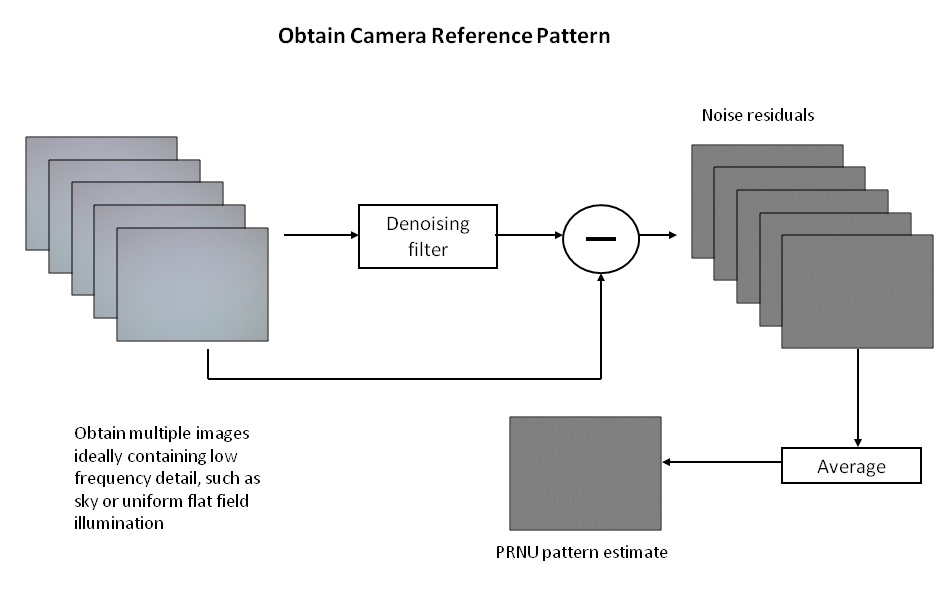
\includegraphics[width=0.4\textwidth]{images/prnu_extraction.jpg}
\end{center}
  \caption{La fase di estrazione del \emph{reference pattern} di una sorgente\cite{figprnu}}
\label{fig:extraction}
\end{figure}

L'implementazione delle funzioni per l'estrazione del PRNU da una singola immagine e per l'estrazione della \emph{fingerprint} da un'insieme di immagini è presa da \cite{goljan2016effect}\footnote{\emph{Effect of Compression on Sensor-Fingerprint Based Camera Identification}}.